% Options for packages loaded elsewhere
% Options for packages loaded elsewhere
\PassOptionsToPackage{unicode}{hyperref}
\PassOptionsToPackage{hyphens}{url}
%
\documentclass[
  english,
  russian,
  12pt,
  a4paper,
  DIV=11,
  numbers=noendperiod]{scrreprt}
\usepackage{xcolor}
\usepackage{amsmath,amssymb}
\setcounter{secnumdepth}{5}
\usepackage{iftex}
\ifPDFTeX
  \usepackage[T1]{fontenc}
  \usepackage[utf8]{inputenc}
  \usepackage{textcomp} % provide euro and other symbols
\else % if luatex or xetex
  \usepackage{unicode-math} % this also loads fontspec
  \defaultfontfeatures{Scale=MatchLowercase}
  \defaultfontfeatures[\rmfamily]{Ligatures=TeX,Scale=1}
\fi
\usepackage{lmodern}
\ifPDFTeX\else
  % xetex/luatex font selection
\fi
% Use upquote if available, for straight quotes in verbatim environments
\IfFileExists{upquote.sty}{\usepackage{upquote}}{}
\IfFileExists{microtype.sty}{% use microtype if available
  \usepackage[]{microtype}
  \UseMicrotypeSet[protrusion]{basicmath} % disable protrusion for tt fonts
}{}
\usepackage{setspace}
% Make \paragraph and \subparagraph free-standing
\makeatletter
\ifx\paragraph\undefined\else
  \let\oldparagraph\paragraph
  \renewcommand{\paragraph}{
    \@ifstar
      \xxxParagraphStar
      \xxxParagraphNoStar
  }
  \newcommand{\xxxParagraphStar}[1]{\oldparagraph*{#1}\mbox{}}
  \newcommand{\xxxParagraphNoStar}[1]{\oldparagraph{#1}\mbox{}}
\fi
\ifx\subparagraph\undefined\else
  \let\oldsubparagraph\subparagraph
  \renewcommand{\subparagraph}{
    \@ifstar
      \xxxSubParagraphStar
      \xxxSubParagraphNoStar
  }
  \newcommand{\xxxSubParagraphStar}[1]{\oldsubparagraph*{#1}\mbox{}}
  \newcommand{\xxxSubParagraphNoStar}[1]{\oldsubparagraph{#1}\mbox{}}
\fi
\makeatother


\usepackage{longtable,booktabs,array}
\usepackage{calc} % for calculating minipage widths
% Correct order of tables after \paragraph or \subparagraph
\usepackage{etoolbox}
\makeatletter
\patchcmd\longtable{\par}{\if@noskipsec\mbox{}\fi\par}{}{}
\makeatother
% Allow footnotes in longtable head/foot
\IfFileExists{footnotehyper.sty}{\usepackage{footnotehyper}}{\usepackage{footnote}}
\makesavenoteenv{longtable}
\usepackage{graphicx}
\makeatletter
\newsavebox\pandoc@box
\newcommand*\pandocbounded[1]{% scales image to fit in text height/width
  \sbox\pandoc@box{#1}%
  \Gscale@div\@tempa{\textheight}{\dimexpr\ht\pandoc@box+\dp\pandoc@box\relax}%
  \Gscale@div\@tempb{\linewidth}{\wd\pandoc@box}%
  \ifdim\@tempb\p@<\@tempa\p@\let\@tempa\@tempb\fi% select the smaller of both
  \ifdim\@tempa\p@<\p@\scalebox{\@tempa}{\usebox\pandoc@box}%
  \else\usebox{\pandoc@box}%
  \fi%
}
% Set default figure placement to htbp
\def\fps@figure{htbp}
\makeatother



\ifLuaTeX
\usepackage[bidi=basic,provide=*]{babel}
\else
\usepackage[bidi=default,provide=*]{babel}
\fi
% get rid of language-specific shorthands (see #6817):
\let\LanguageShortHands\languageshorthands
\def\languageshorthands#1{}


\setlength{\emergencystretch}{3em} % prevent overfull lines

\providecommand{\tightlist}{%
  \setlength{\itemsep}{0pt}\setlength{\parskip}{0pt}}



 
\usepackage[style=gost-numeric,backend=biber,langhook=extras,autolang=other*]{biblatex}
\addbibresource{bib/cite.bib}

\usepackage[]{csquotes}

\KOMAoption{captions}{tableheading}
\usepackage{indentfirst}
\usepackage{float}
\floatplacement{figure}{H}
\usepackage{libertine}
\usepackage{indentfirst}
\usepackage{float}
\floatplacement{figure}{H}
\usepackage[math,RM={Scale=0.94},SS={Scale=0.94},SScon={Scale=0.94},TT={Scale=MatchLowercase,FakeStretch=0.9},DefaultFeatures={Ligatures=Common}]{plex-otf}
\makeatletter
\@ifpackageloaded{caption}{}{\usepackage{caption}}
\AtBeginDocument{%
\ifdefined\contentsname
  \renewcommand*\contentsname{Содержание}
\else
  \newcommand\contentsname{Содержание}
\fi
\ifdefined\listfigurename
  \renewcommand*\listfigurename{Список иллюстраций}
\else
  \newcommand\listfigurename{Список иллюстраций}
\fi
\ifdefined\listtablename
  \renewcommand*\listtablename{Список таблиц}
\else
  \newcommand\listtablename{Список таблиц}
\fi
\ifdefined\figurename
  \renewcommand*\figurename{Рисунок}
\else
  \newcommand\figurename{Рисунок}
\fi
\ifdefined\tablename
  \renewcommand*\tablename{Таблица}
\else
  \newcommand\tablename{Таблица}
\fi
}
\@ifpackageloaded{float}{}{\usepackage{float}}
\floatstyle{ruled}
\@ifundefined{c@chapter}{\newfloat{codelisting}{h}{lop}}{\newfloat{codelisting}{h}{lop}[chapter]}
\floatname{codelisting}{Список}
\newcommand*\listoflistings{\listof{codelisting}{Листинги}}
\makeatother
\makeatletter
\makeatother
\makeatletter
\@ifpackageloaded{caption}{}{\usepackage{caption}}
\@ifpackageloaded{subcaption}{}{\usepackage{subcaption}}
\makeatother
\usepackage{bookmark}
\IfFileExists{xurl.sty}{\usepackage{xurl}}{} % add URL line breaks if available
\urlstyle{same}
\hypersetup{
  pdftitle={Лабораторная работа №4},
  pdfauthor={Перфилов Александр Константинович \textbar{} группа НПИбд 03-24},
  pdflang={ru-RU},
  hidelinks,
  pdfcreator={LaTeX via pandoc}}


\title{Лабораторная работа №4}
\usepackage{etoolbox}
\makeatletter
\providecommand{\subtitle}[1]{% add subtitle to \maketitle
  \apptocmd{\@title}{\par {\large #1 \par}}{}{}
}
\makeatother
\subtitle{Работа с програмными пакетами}
\author{Перфилов Александр Константинович \textbar{} группа НПИбд 03-24}
\date{}
\begin{document}
\maketitle

\renewcommand*\contentsname{Содержание}
{
\setcounter{tocdepth}{1}
\tableofcontents
}
\listoffigures
\listoftables

\setstretch{1.5}
\chapter{Цель
работы}\label{ux446ux435ux43bux44c-ux440ux430ux431ux43eux442ux44b}

\begin{itemize}
\tightlist
\item
  Получить навыки работы с репозиториями и менеджерами пакетов.
\end{itemize}

\chapter{Работа с
репозиториями}\label{ux440ux430ux431ux43eux442ux430-ux441-ux440ux435ux43fux43eux437ux438ux442ux43eux440ux438ux44fux43cux438}

Переходим в пользовательскую учетную запись root с помощью su -

\begin{figure}

{\centering 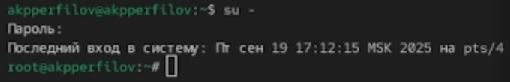
\includegraphics[width=0.71\linewidth,height=\textheight,keepaspectratio]{image/1.jpg}

}

\caption{переходим в уч запись root}

\end{figure}%

Переходим в каталог etc/yum.repos.d и изучаем

Переходим в каталог /etc/yum.repos.d и изучаем информацию о них с
помощью ls и cat название\_репозитория.repo

\begin{figure}

{\centering 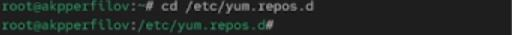
\includegraphics[width=0.2\linewidth,height=\textheight,keepaspectratio]{image/2.jpg}

}

\caption{переходим в repos.d}

\end{figure}%

\begin{figure}

{\centering 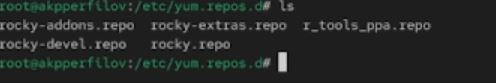
\includegraphics[width=0.2\linewidth,height=\textheight,keepaspectratio]{image/3.jpg}

}

\caption{ищем информацию с помощбю ls}

\end{figure}%

\begin{figure}

{\centering 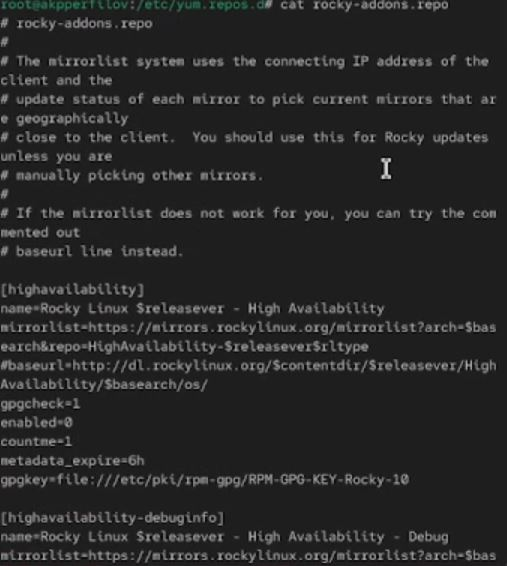
\includegraphics[width=0.2\linewidth,height=\textheight,keepaspectratio]{image/4.jpg}

}

\caption{узнаем подробную информацию с помощью cat}

\end{figure}%

Выводим на экран список репозиториев

Выведем списки репозиториев и получили appstream - для стандартных
приложений baseos - для комппьютерной системы extras - для всего кроме
стандартных приложений и компьютерной системы

\begin{figure}

{\centering 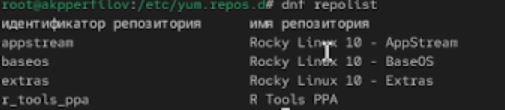
\includegraphics[width=0.71\linewidth,height=\textheight,keepaspectratio]{image/5.jpg}

}

\caption{создаем списки репозиториев}

\end{figure}%

Ищем в каких пакетах есть слово user

С помощью команды dnf search user ищем пакеты в которых присутствует
слово user

\begin{figure}

{\centering 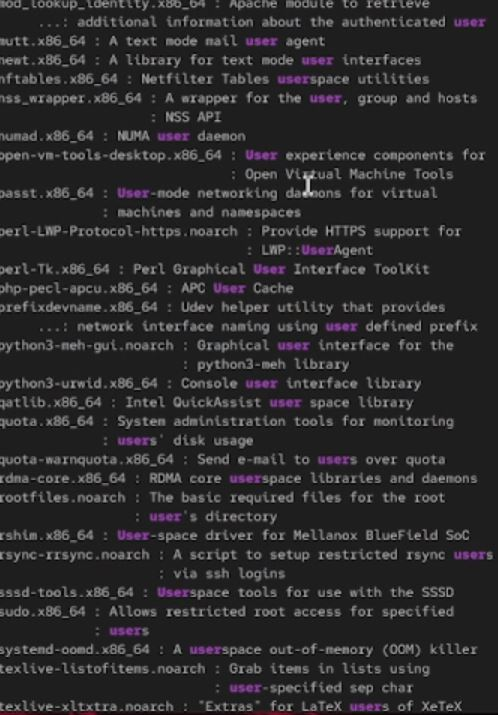
\includegraphics[width=0.71\linewidth,height=\textheight,keepaspectratio]{image/6.jpg}

}

\caption{ищем все пакеты где есть слово user}

\end{figure}%

Устанавливаем nmap

Проверяем информацию о nmap и устанавливаем nmap

\begin{figure}

{\centering 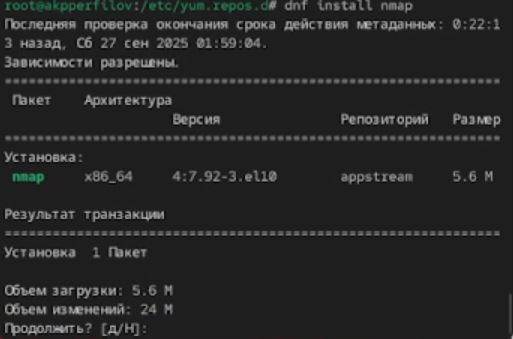
\includegraphics[width=0.3\linewidth,height=\textheight,keepaspectratio]{image/7.jpg}

}

\caption{устанавливаем nmap}

\end{figure}%

Устанавливаем nmap*

\begin{figure}

{\centering 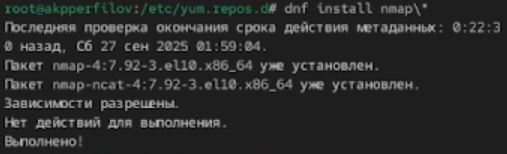
\includegraphics[width=0.3\linewidth,height=\textheight,keepaspectratio]{image/8.jpg}

}

\caption{устанавливаем nmap*}

\end{figure}%

nmap устанавливает конкретный пакет nmap а nmap* устанавливает все что
начинается на nmap

Удаляем nmap и nmap*

\begin{figure}

{\centering 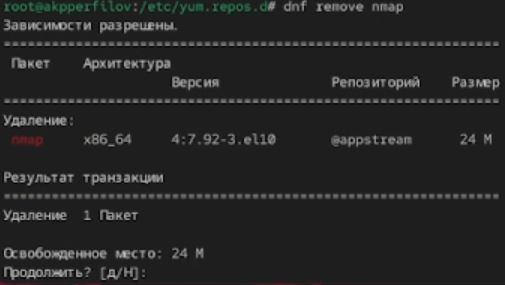
\includegraphics[width=0.3\linewidth,height=\textheight,keepaspectratio]{image/9.jpg}

}

\caption{удаляем nmap}

\end{figure}%

\begin{figure}

{\centering 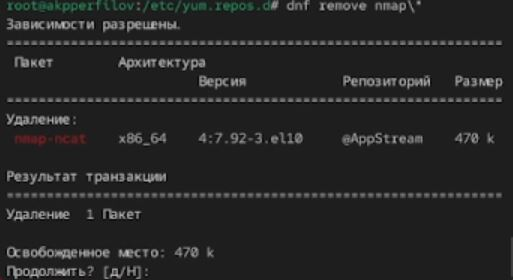
\includegraphics[width=0.3\linewidth,height=\textheight,keepaspectratio]{image/10.jpg}

}

\caption{удаляем nmap*}

\end{figure}%

Устанавливаем группу пакетов RPM Development Tools

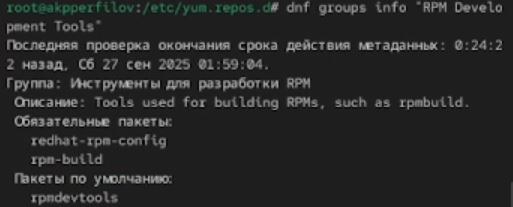
\includegraphics[width=0.2\linewidth,height=\textheight,keepaspectratio]{image/11.jpg}

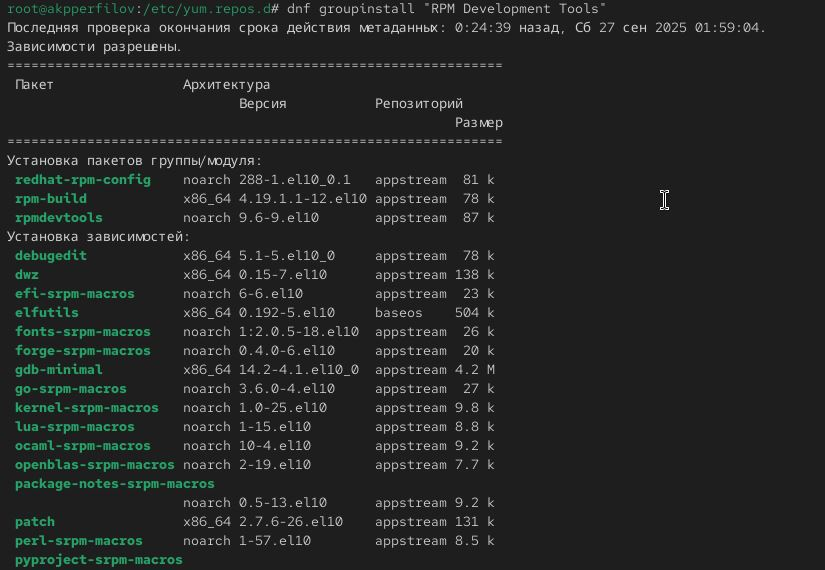
\includegraphics[width=0.2\linewidth,height=\textheight,keepaspectratio]{image/12.jpg}

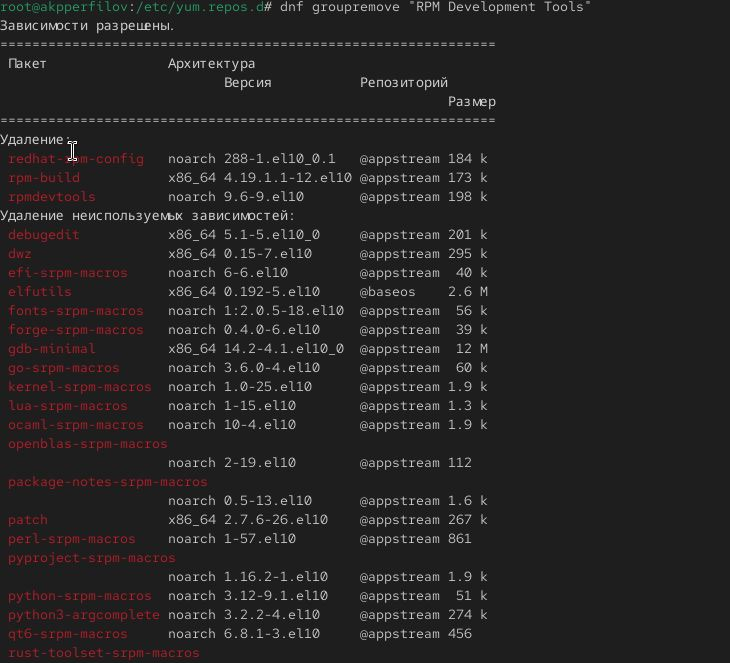
\includegraphics[width=0.2\linewidth,height=\textheight,keepaspectratio]{image/13.jpg}

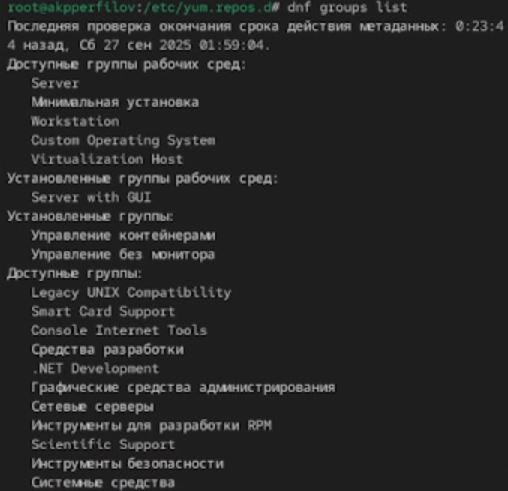
\includegraphics[width=0.2\linewidth,height=\textheight,keepaspectratio]{image/14.jpg}

Удаляем ранее установленные пакеты RPM Development Tools

\begin{figure}

{\centering 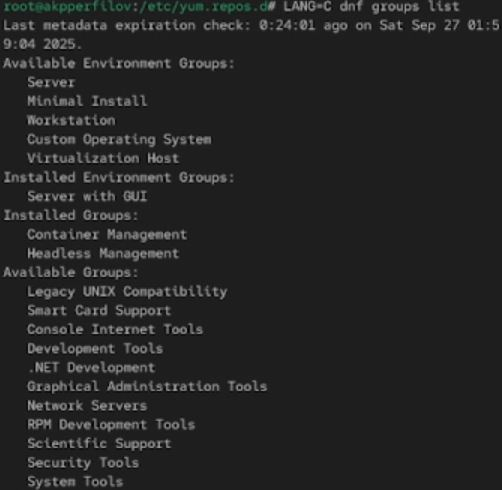
\includegraphics[width=0.71\linewidth,height=\textheight,keepaspectratio]{image/15.jpg}

}

\caption{удаляем RPM Development Tools}

\end{figure}%

Смотрим информацию где и сколько раз использовался dnf

\begin{figure}

{\centering 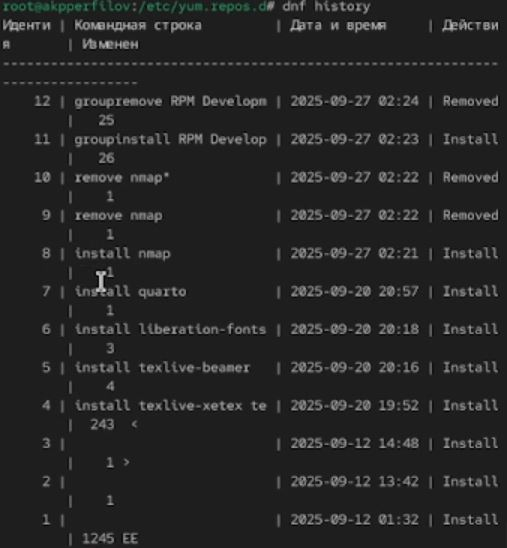
\includegraphics[width=0.71\linewidth,height=\textheight,keepaspectratio]{image/16.jpg}

}

\caption{проверяем dnf}

\end{figure}%

\begin{itemize}
\tightlist
\item
  Отменяем последнее действие с dnf с помощью dnf history undo
\end{itemize}

\begin{figure}

{\centering 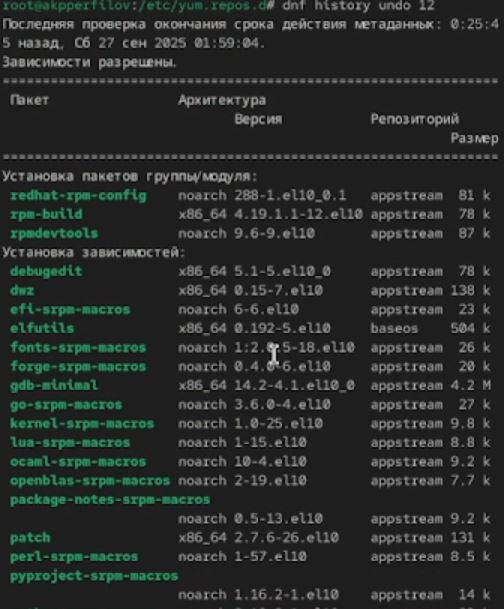
\includegraphics[width=0.71\linewidth,height=\textheight,keepaspectratio]{image/17.jpg}

}

\caption{отменяем последнее действиее 12 с dnf}

\end{figure}%

Качаем группу rpm lynx

\begin{figure}

{\centering 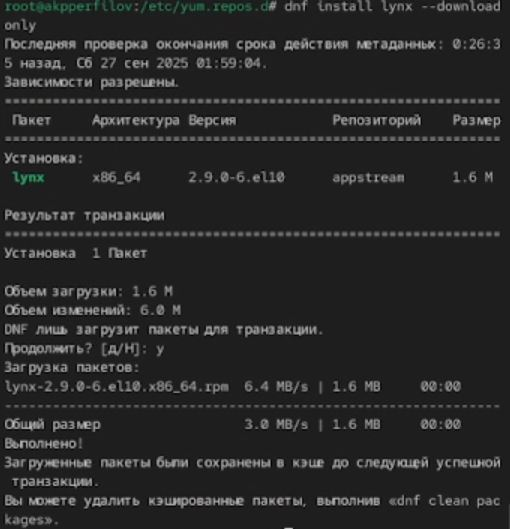
\includegraphics[width=0.71\linewidth,height=\textheight,keepaspectratio]{image/18.jpg}

}

\caption{скачиваем rpm lynx}

\end{figure}%

Находим наш пакет в каталогах

\begin{figure}

{\centering 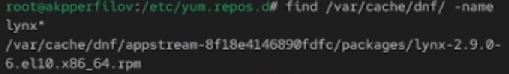
\includegraphics[width=0.71\linewidth,height=\textheight,keepaspectratio]{image/19.jpg}

}

\caption{ищем lynx в каталоге}

\end{figure}%

Переходим в каталог в котом находится lynx

\begin{figure}

{\centering 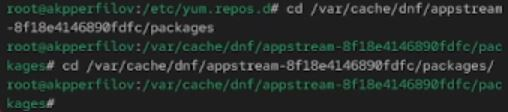
\includegraphics[width=0.71\linewidth,height=\textheight,keepaspectratio]{image/20.jpg}

}

\caption{переходим в каталог где lynx}

\end{figure}%

Устанавливаем rpm пакет в каталоге в ктором находится lynx

\begin{figure}

{\centering 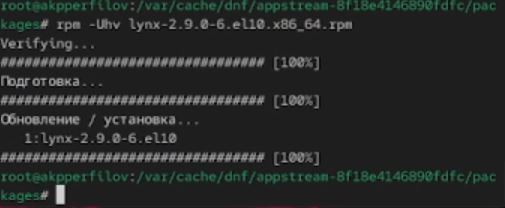
\includegraphics[width=0.71\linewidth,height=\textheight,keepaspectratio]{image/21.jpg}

}

\caption{устанавливаем rpm в каталог с lynx}

\end{figure}%

Определяем расположение файла с помощью команды which lynx

\begin{figure}

{\centering 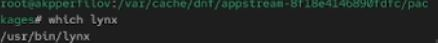
\includegraphics[width=0.71\linewidth,height=\textheight,keepaspectratio]{image/22.jpg}

}

\caption{определяем расположение файла lynx}

\end{figure}%

С помощью rpm определяем к какому пакету принадлежит lynx

\begin{figure}

{\centering 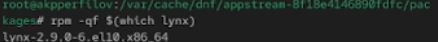
\includegraphics[width=0.3\linewidth,height=\textheight,keepaspectratio]{image/23.jpg}

}

\caption{определяем к какому пакету принадлежит lynx}

\end{figure}%

Получаем доп информацию с помощью rpm -qi lynx

\begin{figure}

{\centering 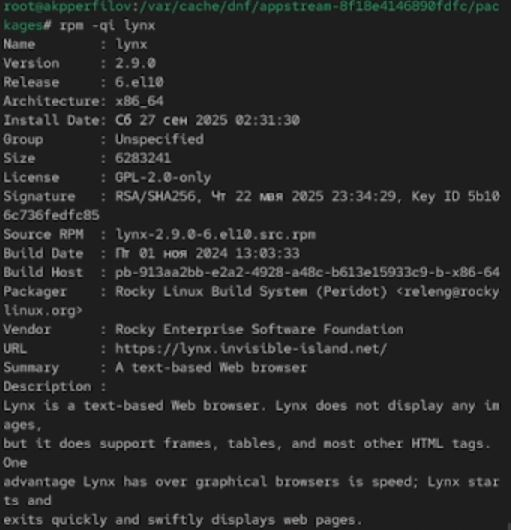
\includegraphics[width=0.3\linewidth,height=\textheight,keepaspectratio]{image/24.jpg}

}

\caption{получаем дополнительную информацию}

\end{figure}%

Получаем список всех файлов в пакете

\begin{figure}

{\centering 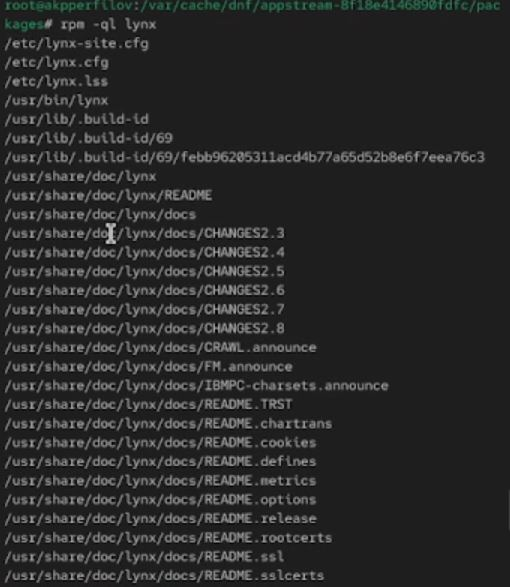
\includegraphics[width=0.2\linewidth,height=\textheight,keepaspectratio]{image/25.jpg}

}

\caption{список всех файлов}

\end{figure}%

Получаем перечень файлов с документацией пакета

\begin{figure}

{\centering 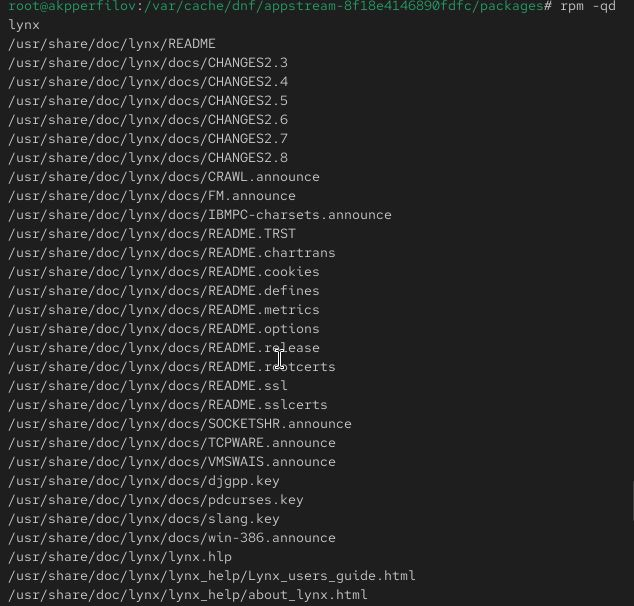
\includegraphics[width=0.2\linewidth,height=\textheight,keepaspectratio]{image/26.jpg}

}

\caption{перечень файлов с документацией пакета}

\end{figure}%

С помощью команды man lynx смотрим файлы документации

\begin{figure}

{\centering 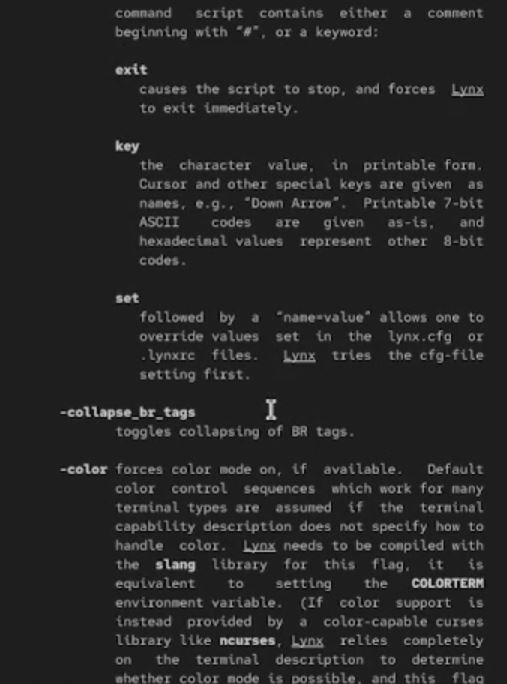
\includegraphics[width=0.2\linewidth,height=\textheight,keepaspectratio]{image/27.jpg}

}

\caption{смотрим файлы документации}

\end{figure}%

Выводим на экран перечень и местоположение конфигурационных файлов
пакета

\begin{figure}

{\centering 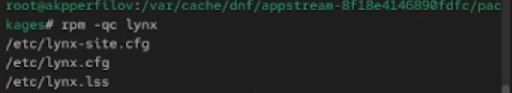
\includegraphics[width=0.71\linewidth,height=\textheight,keepaspectratio]{image/28.jpg}

}

\caption{выводим на экран перечень и местоположение файлов пакета}

\end{figure}%

Находим расположение и содержание скриптов и видим что скриптов у нас
нету

\begin{figure}

{\centering 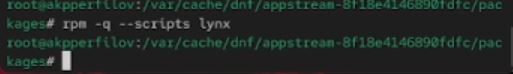
\includegraphics[width=0.71\linewidth,height=\textheight,keepaspectratio]{image/29.jpg}

}

\caption{находим скрипты}

\end{figure}%

Переходим в отдельный терминал и под своей учетной записью запускаем
lynx

\begin{figure}

{\centering 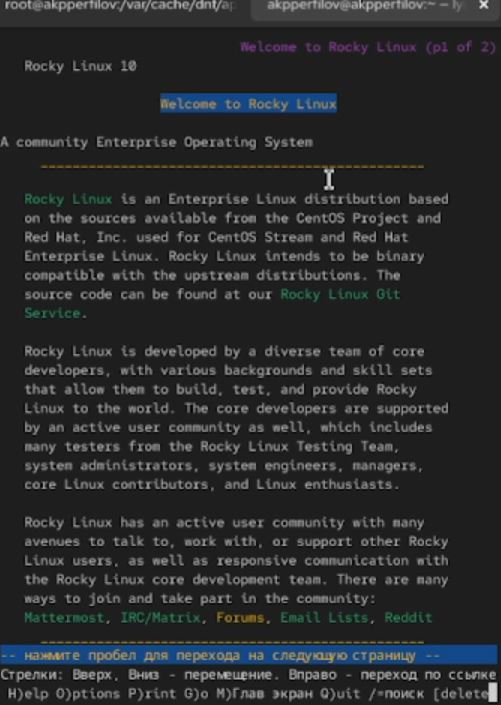
\includegraphics[width=0.71\linewidth,height=\textheight,keepaspectratio]{image/30.jpg}

}

\caption{запускаем lynx}

\end{figure}%

Возвращаемся в терминал root и удаляем пакеты lynx

\begin{figure}

{\centering 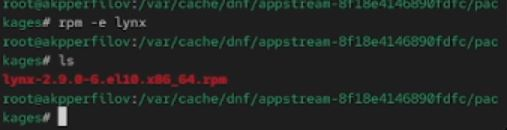
\includegraphics[width=0.71\linewidth,height=\textheight,keepaspectratio]{image/31.jpg}

}

\caption{удаляем lynx}

\end{figure}%

Устанавливаем пакеты dnsmasq

\begin{figure}

{\centering 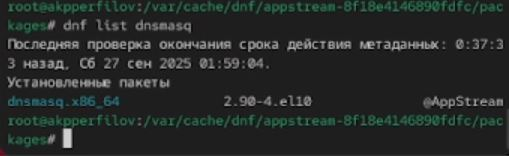
\includegraphics[width=0.3\linewidth,height=\textheight,keepaspectratio]{image/32.jpg}

}

\caption{качаем dnsmasq}

\end{figure}%

Определяем расположение файла с помощью which dnsmasq

\begin{figure}

{\centering 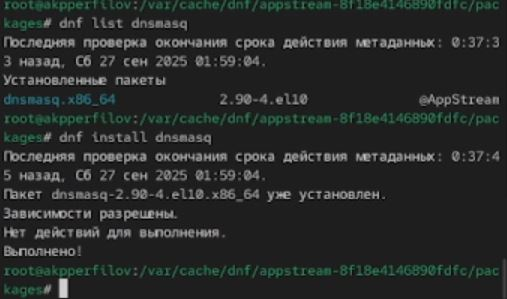
\includegraphics[width=0.3\linewidth,height=\textheight,keepaspectratio]{image/33.jpg}

}

\caption{ищем расположение файла dnsmasq}

\end{figure}%

Определяем к какому пакету принадлежит dnsmasq

\begin{figure}

{\centering 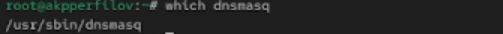
\includegraphics[width=0.3\linewidth,height=\textheight,keepaspectratio]{image/34.jpg}

}

\caption{определяем где dnsmasq}

\end{figure}%

Получаем доп информацию о содержимом пакета

\begin{figure}

{\centering 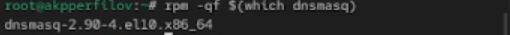
\includegraphics[width=0.3\linewidth,height=\textheight,keepaspectratio]{image/35.jpg}

}

\caption{получаем дополнительную информацию о содержимом пакета}

\end{figure}%

Получаем список всех файлов в пакете dnsmasq

\begin{figure}

{\centering 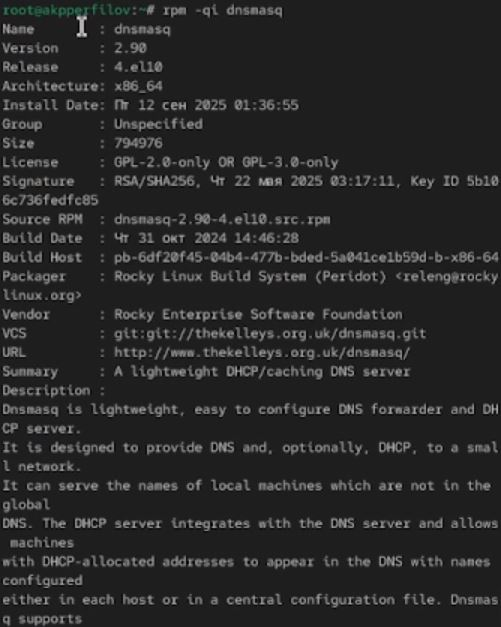
\includegraphics[width=0.71\linewidth,height=\textheight,keepaspectratio]{image/36.jpg}

}

\caption{получаем список всех файлов в пакете}

\end{figure}%

Выводи перечень файлов с документацией пакета dnsmasq

\begin{figure}

{\centering 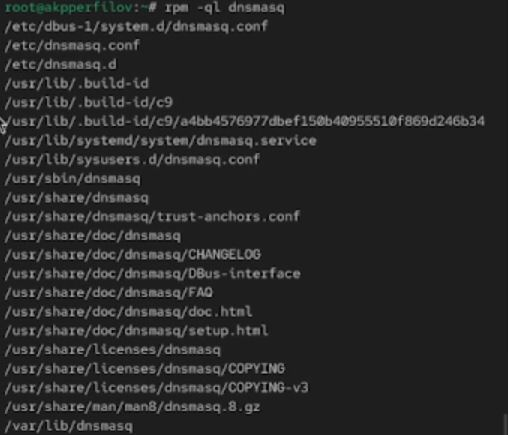
\includegraphics[width=0.71\linewidth,height=\textheight,keepaspectratio]{image/37.jpg}

}

\caption{Получаем документацию пакета dnsmasq}

\end{figure}%

Выводи на экран перечень и месторасположение конфигурационных файлов
пакета

\begin{figure}

{\centering 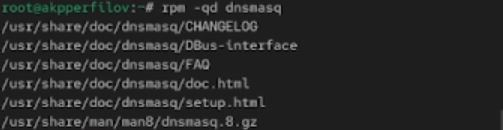
\includegraphics[width=0.71\linewidth,height=\textheight,keepaspectratio]{image/38.jpg}

}

\caption{выводим файлы пакета}

\end{figure}%

Выводим на экран расположение и содержание скриптов

\begin{figure}

{\centering 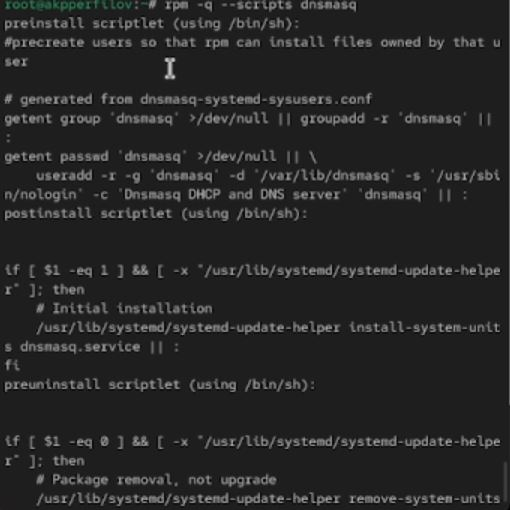
\includegraphics[width=0.71\linewidth,height=\textheight,keepaspectratio]{image/41.jpg}

}

\caption{выводим скрипты}

\end{figure}%

все эти скрипты создаются при пользователе

Возвращаемся в терминал root и удаляем пакет rpm -e dnsmasq

\begin{figure}

{\centering 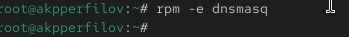
\includegraphics[width=0.71\linewidth,height=\textheight,keepaspectratio]{image/последний.jpg}

}

\caption{удаляем dnsmasq}

\end{figure}%

\chapter{Вывод:}\label{ux432ux44bux432ux43eux434}

В ходе работы приобретены умения по работе с репозиториями и менеджарами
пакетов а также поиску информации о них


\printbibliography



\end{document}
